\documentclass[a5paper,titlepage,11pt,openany]{scrbook}
\usepackage[a5paper,backref]{hyperref}
\usepackage[papersize={148.5mm,215mm},twoside,bindingoffset=0.5cm,hmargin={1cm,1cm},
				vmargin={2cm,2cm},footskip=1.1cm,driver=dvipdfm]{geometry}
\usepackage{palatino}
\usepackage[utf8]{inputenc}

\usepackage{pstricks}
\usepackage{graphicx}
\usepackage[bahasa]{babel} 
\usepackage{lettrine}
\usepackage{pifont}
\usepackage{enumitem}
\usepackage{wrapfig}
\usepackage{indentfirst}
\usepackage{parcolumns}
\usepackage[titles]{tocloft}
\usepackage{longtable}
\usepackage{microtype}
\usepackage{hyphenat}
%\usepackage[raggedright]{titlesec}
%\usepackage{titletoc}


\renewcommand{\cftchapfont}{%
  \fontsize{9}{8}\selectfont
}

\makeatletter
\renewcommand{\@pnumwidth}{1em} 
\renewcommand{\@tocrmarg}{1em}
\makeatother

\author{Lingkungan St. Petrus Maguwo}
\title{Warta Iman}
\setlength{\parindent}{1cm}
\psset{unit=1mm}


\begin{document}
\thispagestyle{empty}
\thispagestyle{empty}
\newcommand{\edisi}[1]{%
\DeclareFixedFont{\PT}{T1}{ppl}{b}{}{0.7in}
\DeclareFixedFont{\PTit}{T1}{ppl}{b}{it}{0.7in}
\DeclareFixedFont{\PTsmall}{T1}{ppl}{b}{it}{0.25in}
\DeclareFixedFont{\PTsmaller}{T1}{ppl}{b}{it}{0.175in}
\DeclareFixedFont{\PTsmallest}{T1}{ppl}{b}{it}{0.15in}

\begin{pspicture}(14cm,2cm)
\rput[rb](10.35cm,3cm){\PTsmallest {#1}}
\rput[lb](-2cm,1.5cm){\PT {WARTA IMAN}}
\rput[lb](0cm,0.5cm){\PTsmall {Lingkungan St. Petrus Maguwo}}
\end{pspicture}%
}

\newcounter{kgkcounter}[chapter]
\renewcommand{\thekgkcounter}{\arabic{kgkcounter}. }
\newcommand{\kgk}[1]{\refstepcounter{kgkcounter}\textbf{\flushleft \textbf{\thekgkcounter #1}}\\}

\newcommand{\kutipan}[1]{%
\noindent{\framebox{\parbox{10cm}{\centering\emph{#1}}}}}

\edisi{November 2011}

%\vspace{1cm}

\begin{center}
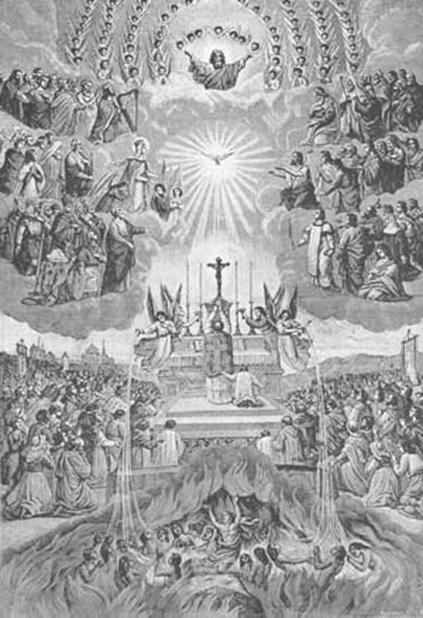
\includegraphics[scale=0.85]{gambar/purgatory2.jpg}
\end{center}

%\vspace{1cm}

\begin{center}
{\PTsmaller {Kasih, kerendahan hati, dan menurut pada kehendak Allah }}
\end{center}

\setlength{\parindent}{1cm}
\pagestyle{plain}
\chap{Sakramen Imamat dan Hidup Menjadi Imam}
Sakramen Imamat sering disebut dengan Sakramen Tahbisan = Sakramen Wisuda. Dengan Tahbisan, seseorang menjadi Pemimpin dalam Gereja. Dulu pernah salah dipahami bahwa Sakramen Imamat/Tahbisan ini hanya untuk Pemimpin Ekaristi – memberi absolusi dalam Sakramen Tobat saja. Dengan Sakramen Imamat seseorang diangkat / diwisuda untuk menggembalakan Gereja dengan Sabda \& Roh Allah

Yang bisa menerima Sakramen Imamat adalah
semua orang pria/laki-laki yang tidak terikat pernikahan, yang beragama / iman Katolik
    Dewasa dalam kepribadian -- iman
    Telah mendapatkan pendidikan cukup di Seminari Tinggi

Ordo dalam arti luas: Ordo berarti lembaga religius, sehingga mencakup baik Ordo dengan kaul agung maupun konggregasi \& serikat hidup kerasulan dengan kaul sederhana. Dalam arti sempit: Ordo berarti lembaga religius / persekutuan yang anggotanya pria atau wanita. Imam atau awam mengikrarkan ketiga nasihat Injil sebagai kaul kekal yang publik serta meriah (atau agung) \& hidup dalam persaudaraan. Tujuannya membuktikan diri kepada Tuhan. Para Imam/Biarawan/Biarawati mengucapkan 3 kaul:
\begin{enumerate}
\item Kaul Ketaatan
\item Kaul Kemiskinan
\item Kaul Kemurnian
\end{enumerate}

Waktu yang diperlukan seseorang menjalani sekolah Seminari sampai akhirnya bisa disebut Frater (mulai dari proses pendaftaran sampai masuk Seminari / tahapan menjadi seorang Frater)
antara 7-8 tahun dengan pentahapan

\begin{itemize}
\item Tahap Postulat: 1 thn
\item Tahap Novis: 1 thn
\item Tahap Filosofan (studi Filsafat): 3 thn
\item Tahap Toper (praktek pastoral di Paroki): 1-2 thn
\item Tahap Teologan (studi Teologi): 2 thn
\item Tahap Diakonat: +/- 6 bulan di Paroki lagi(Diakon sudah termasuk Klerus, artinya bukan awam, karena sudah ditahbiskan sebagai Diakon)
\end{itemize}

Mulai tahap Novislat s/d Skolastikat disebut Frater. Mulai tingkat 5 diperbolehkan mengucapkan kaul kekal. Sebelumnya hanya kaul sementara (1 thn, 2 thn – 3 thn). Setelah kaul kekal lalu mendapatkan tahbisan Diakon, lalu Pastoral di Paroki 6 bulan disusul Tahbisan.

Liburan diatur menurut ketentuan Keuskupan masing-masing ada yang
\begin{itemize}
\item 3 thn mendapatkan libur/cuti 1 bulan
\item 2 thn mendapatkan libur/cuti 2 bulan
\item 1 thn mendapatkan libur/cuti 1 bulan
\item Libur Semester sesuai kalendar akademik masing-masing seminari.
\end{itemize}

Kegiatan yang dilakukan oleh Imam sehari-harinya adalah
memimpin/menggembalakan Jemaat di Paroki

\begin{itemize}
\item melayani Sakramen (7 Sakramen)
\item Doa Pribadi
\item Ada yang jadi dosen/ketua yayasan
\item Bidang sosial
\end{itemize}

Lalu, seberapa pentingnya kah DOA dalam kehidupan sehari-hari seorang Imam?
Romo: Doa menjadi tiang penyangga utama seorang Imam, khususnya dalam Perayaan Ekaristi, tapi juga doa-doa harian pribadi – renungan Kitab Suci. Juga bagi kaum awam sangat penting.

Saat menjadi frater mempunyai tugas pokok: studi, ada tugas tambahan: mengajar agama di sekolah, memberi Retreat -- Rekoleksi kaum muda, latihan-latihan pastoral  semuanya dalam bimbingan Pastor Rektor Seminari / staff.
Frater juga melakukan rekreasi dan kerja tangan.

Pemenuhan/perolehan Sakramen Imamat merupakan puncak kerinduan seorang Calon Imam. Tapi menjadi imam adalah panggilan Tuhan (banyak yang dipanggil, sedikit yang dipilih). Orang harus selalu membuka hati bagi panggilan Tuhan, bersedia meninggalkan kepentingan-kepentingan pribadi untuk bisa mengabdi / melayani Tuhan / Gereja / umatNya.

Para Uskup memakai cincin sebagai tanda bahwa dia Uskup. Uskup juga Tahbisan, justru ini tahbisan tertinggi (tingkat 1). Imam/Pastor adalah tahbisan di bawahnya (tingkat II). 

\begin{quote}\emph{
LG 21: Sebab dengan tahbisan Uskup diterimakan kepenuhan Sakramen Imamat yang biasanya disebut Imamat Tertinggi atau keseluruhan pelayanan suci. Adapun para imam biasa kendatipun tidak menerima puncak imamat dan dalam melaksanakan kuasa mereka tergantung ari para Uskup, namun mereka sama-sama imam seperti para Uskup \& berdasarkan Sakramen Tahbisan merekapun dikhususkan untuk mewartakan Injil serta menggembalakan umat beriman \& untuk merayakan Ibadah Ilahi sebagai Imam sejati perjanjian baru (1628). Akhirnya masih ada para Diakon yang juga ditumpangi tangan tapi bukan untuk Imamat melainkan untuk pelayanan. (1629).}
\end{quote}

Jadi, ada 3 macam Sakramen Tahbisan:
\begin{enumerate}
\item Tahbisan Uskup
\item Tahbisan Imam
\item Tahbisan Diakon
\end{enumerate}

\sumber{nara sumber: Pastor Josef Kristianto}
\vfill
\noindent{\framebox{\parbox{11cm}{\centering\emph{
”Keluarga-keluarga tidak hanya menjadi tempat istimewa untuk membentuk jati diri manusiawi dan kristiani, tetapi juga menjadi “lahan penyemaian benih-benih panggilan yang utama dan terbaik bagi hidup yang dibaktikan demi Kerajaan Allah” (Familiaris Consortio, 53), dengan membantu anggota-anggotanya melihat secara tepat di dalam keluarga itu sendiri, keindahan dan pentingnya imamat dan hidup bakti. 
{~}\\
Para imam dan seluruh kaum beriman awam hendaknya selalu bekerja sama, agar di dalam Gereja semakin berlipat-ganda “rumah-rumah dan sekolah-sekolah persekutuan” yang menjadi cerminan harmonis persekutuan Tritunggal Mahakudus di dunia ini, seturut teladan Keluarga Kudus Nazaret.”}\\
(Pesan Bapa Suci untuk Hari Doa Panggilan Sedunia ke-49)
} } }

\chap{Kami mengasihimu, pastor!}

\section*{Pendahuluan}

Ada suatu percakapan antara dua orang ibu, Tina dan Suti. Tina bertanya kepada Suti “\textit{Anak kamu kalau sudah besar ingin menjadi apa?}” Suti menjawab, "\textit{Anakku ingin menjadi dokter bedah. Bagaimana dengan anak kamu yang selalu juara, Tina?}” Kemudian Tina menjawab “Anakku ingin menjadi pastor.” Suti terdiam, dan perlahan-lahan berkata “\textit{Ehm \ldots sayang juga ya, pintar-pintar kok mau jadi pastor.}”

Disinikah kita melihat, seolah-olah kalau yang bagus dan baik, jangan menjadi pastor. Padahal kita melihat di Alkitab bahwa hanya yang terbaik sajalah yang dipersembahkan kepada Allah. Kita melihat bagaimana pemilihan kurban bakaran selalu memilih kurban yang terbaik (Im 14:10). Minyak yang dipakai di bait Allah, juga minyak yang terbaik (Bil 18:12). Hanya yang terbaiklah yang dapat kita persembahkan kepada Tuhan, termasuk imam.

Kalau kita renungkan, kita dapat mengatakan bahwa keberhasilan suatu paroki dalam membina umatnya dapat diukur dari berapa banyak kaum muda yang menjawab panggilan menjadi pastor dari paroki yang bersangkutan. Semakin baik kehidupan spiritual paroki tersebut, maka akan semakin banyak kaum muda yang terpanggil menjadi pastor, karena keinginan untuk menjadi pastor dimulai dari keluarga dan juga dari lingkungan gereja. Jadi hal pertama yang perlu kita renungkan adalah: \textbf{berapakah yang menjadi pastor dari parokiku?} Kalau jawabannya tidak ada, maka perlu dipikirkan bagaimana untuk menggalakkan panggilan, sehingga putera-puteri yang terbaik dari paroki masing-masing dapat menjadi pastor atau suster.

\section*{Bukan engkau yang memilih-Ku, namun Aku yang memilihmu}

Namun yang terbaik menurut ukuran kita, bukanlah yang terbaik untuk ukuran Tuhan. Jadi, kalau mau ditanya siapa yang layak untuk menjadi pastor? Jawabnya adalah “tidak ada yang layak.” Namun, di tengah ketidaklayakan inilah, Tuhan memilih mereka, sama seperti Tuhan memilih Daud (1 Sam 16:6-13). Nabi Samuel berfikir dan ingin mengambil keputusan berdasarkan penilaian panca indera. Namun dikatakan bahwa Tuhan melihat hati. Dan karena inilah, Tuhan memilih Daud, seorang yang berkenan di hati-Nya(1 Sam 13:14).

\section*{Imam dengan segala suka dukanya}

Mungkin kita sering melihat ada beberapa imam yang sudah ditahbiskan yang tidak memberikan contoh yang baik kepada umatnya. Dan kita sering mengatakan bahwa mereka juga manusia biasa, yang tidak lepas dari dosa. Hal ini memang ada benarnya, sama seperti para rasul yang dipilih oleh Yesus sendiri, mereka juga manusia biasa, sederhana, namun dipilih oleh Tuhan secara khusus menjadi rasul. Apakah semua rasul-Nya setia? Tidak, karena Yudas terbukti menghianati Yesus. Demikian juga dengan para imam jabatan (pastor), yang dipilih oleh Tuhan secara khusus, ada dari mereka yang karena kelemahan mereka tidak dapat berpartisipasi secara baik dalam imamat Kristus. Namun apakah semuanya atau banyak imam yang demikian? Tentu tidak! Bahkan kita dapat melihat betapa banyak imam yang hidupnya tulus dan sungguh menjadi cerminan kasih Kristus. Mereka adalah tanda kehadiran Kristus yang menyertai Gereja-Nya dan pengorbanan mereka sungguh menjadi teladan bagi kita untuk juga mau berkorban dan menyerahkan diri kepada sesama.

Mari kita renungkan sejenak, kalau melihat takaran dunia, apa yang menarik dari kehidupan para imam? Mereka tidak boleh menikah, diberi uang saku ala kadarnya, harus menuruti perintah atasan. Kalau mereka sudah hidup baik dan menyesuaikan diri dengan orang-orang di parokinya, maka atasannya memindahkan mereka, bahkan kadang ke tempat yang terpencil, yang tidak ada listrik dan transportasi yang mencukupi. Kalau mereka tinggal di dalam komunitas, mereka tidak dapat memilih teman satu rumahnya, sedangkan kita minimal masih dapat memilih teman hidup. Kalau mereka jarang ngobrol dengan umat, dibilang pastornya menjaga jarak, namun kalau pastornya akrab dengan umat, dibilang bahwa pastornya cari perhatian atau malah digosipin dekat dengan seseorang. Kalau ada yang sakit parah, maka pastor harus bergegas memberikan sakramen perminyakan orang sakit, tidak peduli jam berapa. Bukankah serba susah untuk menjadi pastor? Kadang saya pikir-pikir, pelayanan ini jauh lebih sulit daripada orang yang bekerja di kantor. Apa rahasianya, sehingga mereka dapat melakukan hal yang demikian? Ya, karena rahmat dan kasih Allah! Dan memang, tanpa mengandalkan rahmat kasih Allah itu, sungguh sangat sulit untuk menjadi pastor. Tetapi bersama Allah, lihatlah, betapa indah dan ajaibnya buah hasil kerja mereka: banyak orang dapat menyadari akan kehadiran Allah yang hidup. Banyak orang tergerak untuk mengenal dan mengasihi Allah, yang mengantar mereka kepada keselamatan kekal! Manusia biasa tak akan sanggup melakukan hal ini, sebab urusan mengubah hati itu hanya pekerjaan Tuhan, namun berbahagialah para pastor yang dipakai Allah untuk menjadi alat-Nya yang istimewa untuk pekerjaan Tuhan ini.

Syukur kepada Tuhan, di tengah-tengah tantangan yang besar ini, banyak kaum muda yang menjawab panggilan Tuhan ini dengan besar hati. Memang, para imam hanya dapat bertahan kalau mereka benar-benar menyadari akan hakikat mereka sebagai orang-orang pilihan Tuhan. Sama seperti sakramen perkawinan yang hanya dapat bertahan jika suami istri mempunyai komunikasi yang baik, demikian juga dengan Sakramen Imamat, para pastor akan bertahan dalam berkat imamatnya, kalau mereka mereka mempunyai komunikasi yang baik dengan Tuhan. Tanpa bertekun dalam doa, dan berani memberikan dirinya untuk orang lain, maka pastor tidak akan dapat memenuhi pelayanannya sesuai dengan yang Tuhan percayakan kepada mereka.

\section*{Imam bersama dan Imam tertahbis}

Mari sekarang kita melihat hakikat dari Sakramen Imamat. Seperti yang kita tahu, bahwa dengan Sakramen Baptis, kita semua menjadi imam, nabi, dan raja. Walaupun panggilan sebagai imam belaku untuk semua yang sudah dibaptis, namun Tuhan menunjuk orang-orang pilihan-Nya untuk menjadi \textbf{imam tertahbis} (imamat jabatan).

\subsection*{Dalam Perjanjian Lama}

Kel 19:5-6, menyatakan bahwa Tuhan memerintahkan Musa untuk memberitahukan kepada seluruh umat Israel, bahwa kalau mereka berpegang pada perintah Tuhan, mereka akan menjadi umat kesayangan, kerajaan imam dan bangsa yang kudus. Di samping mengangkat Israel sebagai kerajaan imam, Perjanjian Lama juga mengatakan bahwa suku Lewi dipersiapkan secara khusus sebagai imam (Bil 3:5-13). Secara umum memang bangsa Israel dipersiapkan Tuhan menjadi imam dan bangsa yang kudus, namun secara khusus, Tuhan juga menunjuk suku Lewi untuk menjadi imam dan menjalankan tugas yang berhubungan dengan korban dan persembahan. Suku Lewi yang ditunjuk secara khusus oleh Tuhan untuk menjadi imam (imamat jabatan) melayani umat yang lain atau imam secara umum (imamat bersama). Hal yang sama dapat diterapkan di dalam ajaran Gereja Katolik. Gereja Katolik mengenal adanya dua imamat: (1) Imamat jabatan dan (2) imamat bersama. Dimana imamat jabatan melayani imamat bersama.[2]

\subsection*{Dalam Perjanjian Baru}

Yesus tidak pernah melarang perantaraan imam sejauh hal tersebut berpartisipasi dalam karya keselamatan Yesus. Pada saat Yesus menyembuhkan sepuluh orang kusta, Yesus menyuruh mereka untuk memperlihatkan diri mereka kepada para imam (Luk 17:12-14) agar para imam dapat menyatakan mereka tahir. Rasul Petrus menegaskan bahwa semua umat Allah adalah bangsa terpilih, imamat yang rajani, bangsa yang kudus, kepunyaan Allah sendiri (1 Pet 2:9). Pemilihan bangsa Israel sebagai bangsa pilihan untuk mendatangkan keselamatan pada bangsa-bangsa lain membuktikan bahwa Tuhan menggunakan ‘perantara’ untuk melaksanakan rencana-Nya.

\section*{Yesus adalah Imam yang sejati dan selamanya}

Dari konsep imam di Perjanjian Lama dan Perjanjian baru, kita melihat bahwa imam di Perjanjian Lama adalah merupakan persiapan untuk imam yang lebih sempurna di Perjanjian Baru, yang dipenuhi di dalam diri Kristus, imam menurut peraturan Melkisedek, yang sempurna, yang berlangsung untuk selamanya (Ibr 5:1-10). Dengan pengorbanan Kristus di kayu salib, maka Yesus telah melengkapi semuanya, baik sebelum kedatangan-Nya, pada waktu kedatangan-Nya, dan setelah kedatangan-Nya. Pertanyaannya, apakah dengan mengakui Yesus sebagai Imam satu-satunya menutup kemungkinan adanya imam yang lain? Sama seperti penjelasan tentang imam jabatan di dalam Perjanjian Baru dan Perjanjian lama, maka \textbf{imam-imam jabatan hanyalah menjadikan Imam yang abadi, yaitu Kristus untuk hadir kembali tanpa menghilangkan keunikan imamat Kristus. Imam-imam yang ditahbiskan hanyalah menjadi pelayan dari Imam satu-satunya, yaitu Kristus.}

Kita dapat melihat bahwa Yesus adalah satu-satunya perantara antara Allah dengan manusia. Jadi doa-doa yang kita panjatkan didaraskan dalam nama Yesus. Namun bukankah kita sering meminta seseorang yang kita anggap punya hubungan baik dengan Tuhan untuk juga mendoakan permasalahan kita? Apakah dengan demikian kita menghilangkan keagungan Yesus yang menjadi satu-satunya Perantara kita dengan Allah? Tentu saja tidak, karena semua orang yang mendoakan kita turut berpartisipasi dalam karya keselamatan Kristus. \textbf{Jadi sampai tahap ini, kita menyetujui bahwa imam yang tertahbis tidak menghilangkan keagungan dan kebenaran bahwa Kristus adalah satu-satunya Imam Agung.}

Dan berdasarkan pembuktian di atas dalam Perjanjian Baru dan Perjanjian Lama, kita tahu bahwa Tuhan telah menjadikan seluruh umat Allah menjadi imam. Namun \textbf{Yesus menunjuk secara khusus imam yang ditahbiskan untuk melanjutkan karya-Nya di dunia ini sampai akhir jaman, dan juga untuk melayani imam bersama.}

\section*{Apakah Sakramen Imamat?}

\subsection*{Imamat jabatan}

Katekismus, 1536 menyebutkan bahwa Tahbisan adalah suatu Sakramen, \textbf{di mana perutusan yang dipercayakan Kristus kepada Rasul-rasul-Nya, dilanjutkan sampai akhir zaman}. Dari sini jelas, bahwa konsep Gereja bukan hanya tak kelihatan, namun juga kelihatan. Namun demikian, hal yang tak terlihat (spiritual) dan terlihat, tak dapat dipisahkan, sama seperti tubuh dan jiwa manusia tak terpisahkan. Dalam hal struktur yang terlihat (Sakramen) ini, terdapat bagian, yaitu: \textbf{episkopat, presbiterat, dan diakonat.}

Episkopat atau uskup adalah penerus dari para rasul, yang diutus oleh Yesus sendiri. Sama seperti Yesus menunjuk rasul Petrus, sebagai kepala dari para murid, maka uskup Roma menjadi penerus dari rasul Petrus menjadi kepala dari seluruh Gereja di seluruh dunia. Sedang para uskup adalah pemimpin dari gereja lokal, yang dibentuk menurut gambaran Gereja universal (semesta) dan dalam kesatuan dengan Bapa Paus. Dan pembantu dari uskup adalah para pastor (presbiterat), yang biasanya membawahi paroki. Sedangkan diakonat diperbantukan untuk membantu pelayanan para pastor dan uskup. Diakonat dan presbiterat ditahbiskan oleh uskup, sedangkan uskup ditahbiskan oleh para uskup yang lain dengan persetujuan dari uskup Roma, atau Paus. \textbf{Dari sinilah, kita melihat bahwa seluruh tahbisan di Gereja Katolik saling terkait dan dapat ditelusuri sampai kepada para Rasul, yang diutus oleh Yesus sendiri}. Karena inilah maka salah satu ciri Gereja Katolik adalah apostolik (berasal dari para Rasul).

\subsection*{Imamat bersama}

\textbf{Pada saat kita dibaptis, maka kita juga dipanggil untuk menjadi imam, nabi dan raja.} Melalui baptisan, kita juga harus menjadi imam, yaitu dengan menjadi saksi Kristus yang baik, hidup menurut iman, pengharapan, dan kasih. Melalui kesaksian hidup kita, maka kita akan menjadi pancaran terang kasih Kristus, sehingga secara tidak langsung, kita berpartisipasi untuk membawa umat yang lain kepada Sang Imam Agung, yaitu Kristus. Dan cara kedua untuk menjalankan imamat bersama adalah dengan mengikuti perayaan Ekaristi. Dimana dengan persiapan, dan partisipasi aktif, kita semua menyatukan persembahan kita, suka duka kita, dan kehidupan kita dalam kurban Ekaristi.

\section*{Imam Jabatan dan Imam bersama berjalan berdampingan untuk membangun Gereja}

Yang menjadi masalah adalah kalau ada orang yang mencoba mencampuradukkan kedua jenis imamat ini. Imam jabatan semakin ingin menyatu dengan umat, dan mengaburkan identitasnya. Dan imam bersama begitu antusias untuk berpartisipasi di pelayanan, sehingga juga mengerjakan pekerjaan-pekerjaan imam jabatan. Padahal, baik imam jabatan maupun imam bersama mempunyai identitas sendiri-sendiri dan keduanya mempunyai tujuan untuk membangun jemaat Allah. Imam bersama terjun ke masyarakat dan menjadi garam di tengah-tengah masyarakat yang nilai-nilainya belum tentu sesuai dengan nilai-nilai kristiani. Sedangkan imam jabatan membangun dan melayani imam bersama, sehingga imam bersama akan semakin dikuatkan untuk menjadi saksi yang hidup di tengah masyarakat.

\section*{Imam Jabatan yang melanjutkan tiga misi Kristus: Imam, Raja, dan Nabi}

\textbf{Sebagai Imam}, para imam melanjutkan karya Kristus dengan merayakan sakramen dan memimpin umat di dalam liturgi, terutama di dalam liturgi Ekaristi. Di sinilah peran imam menjadi begitu jelas, yang mewakili Kristus (persona Christi) untuk menghadirkan kembali kurban Paskah Kristus. Mereka memberikan sakramen Baptis, Penguatan, Pengakuan Dosa, Sakramen Perminyakan, dan memberikan penguburan kepada yang meninggal. Dalam kesehariannya, mereka juga berdoa brevier, doa yang menjadi doa Gereja.

\textbf{Sebagai Nabi}, para imam melaksanakannya dengan berkotbah, mengajar di sekolah atau persiapan Pembaptisan. Secara prinsip seorang pastor harus menyampaikan kebenaran, yang bersumber pada Kitab Suci, Tradisi Suci, dan Magisterium. Imam yang menyampaikan ajaran yang dianggapnya benar namun tidak berdasarkan tiga pilar kebenaran di atas, sebenarnya tidak menjalankan fungsinya sebagai nabi. Karena sebagai nabi, dia hanyalah meneruskan Kebenaran kepada umat, bukan mengarang kebenaran, berdasarkan pendapat pribadi, atau berdasarkan suara umat, karena kebenaran tidak tergantung dari suara terbanyak.

\textbf{Sebagai Raja}, para pastor melaksanakannya dengan pelayanannya di bidang kepemimpinan umat, baik di paroki atau komunitas yang dipercayakan kepada mereka. Mereka bekerja sama dengan dewan paroki, sehingga kegiatan paroki dapat berjalan dengan baik.

\section*{Uskup, Imam, dan diakon menurut Bapa Gereja}

Mungkin ada yang berfikir bahwa uskup, imam dan diakon hanyalah karangan Gereja Katolik semata. Namun kalau kita melihat sejarah dan belajar dari para bapa Gereja, maka kita akan melihat, bahwa sebenarnya semua itu berakar pada tradisi.

\begin{enumerate}
\item \textbf{Ignasius dari Antiokia (AD. 110)}: “Sekarang, sungguh merupakan kehormatan bagiku untuk bertatap muka denganmu secara pribadi dengan uskup (bishop) yang diberkati Tuhan, Damas; dan juga bertemu secara pribadi dengan para imam (presbyters), Bassus dan Apollonius l dan teman satu pelayanan, diakon, Zotion. ..” (Letter to the Magnesians 2).
\item \textbf{Ignasius dari Antiokia (AD. 110)}: “Perhatikanlah untuk melakukan segala sesuatu selaras dengan Tuhan, dengan uskup menempati posisi Tuhan dan dengan para imam di posisi para murid, dan dengan para diakon, yang paling dekat denganku, yang dipercaya dengan pelayanan Kristus, yang berasal dengan Allah Bapa sejak permulaan dan yang pada akhirnya telah dinyatakan (ibid, 6:1).
\item \textbf{Ignasius dari Antiokia (AD. 110)}: “Perhatikanlah, untuk menyelaraskan diri dalam perintah-perintah Allah dan para murid, sehingga di dalam setiap perbuatanmu, kamu dapat berhasil, baik di dalam tubuh maupun jiwa, baik dalam iman dan kasih, dalam Putera, Bapa dan dalam Roh Kudus, di awal dan di akhir, bersama dengan yang terhormat uskupmu; dan dengan para imam, yang terjalin secara baik dalam mahkota rohani; dan dengan para diakon, putera-putera Allah. Tunduklah kepada uskup dan satu sama lain seperti Yesus Kristus taat kepada Allah Bapa, dan para murid kepada Kristus dan Allah Bapa \ldots (ibid, 13:1-2).
\item \textbf{Ignasius dari Antiokia (AD. 110)}: “Memang, engkau harus tunduk kepada uskup seperti engkau tunduk kepada Yesus Kristus, sudahlah jelas bagiku bahwa engkau hidup bukan dengan cara manusia namun di dalam Kristus, yang telah wafat untuk kita… Dengan demikian adalah penting …bahwa engkau tidak melakukan segala sesuatu tanpa persetujuan uskup, dan engkau juga harus tunduk kepada para imam, seperti kepada para murid Kristus…Adalah penting juga bahwa para diakon, pemberi sakramen-sakramen Kristus, dalam segala sesuatu menyenangkan semua orang. .. (Letter to the Trallians 2:1-3).
\item \textbf{Ignasius dari Antiokia (AD. 110)}: ” Setiap orang yang menghormati para diakon menghormati Kristus, dan juga yang menghormati uskup menghormati Allah Bapa, dan menghormati para imam sebagai perwakilan Allah dan persekutuan para murid. Tanpa hal tersebut, maka tidak dapat dikatakan sebuah Gereja. (ibid., 3:1-2).
\item \textbf{Ignasius dari Antiokia (AD. 110)}: “Dia yang ada di dalam tempat kudus adalah kudus; tetapi dia yang berada di luar tempat kudus adalah tidak kudus. Dengan kata lain, seseorang yang bertindak tanpa uskup dan imam dan para diakon tidak mempunyai hati nurani yang bersih” (ibid., 7:2).
\item \textbf{Ignasius dari Antiokia (AD. 110)}: “…saya berbicara dengan suara yang keras, suara dari Tuhan: “Perhatikanlah uskup dan imam dan para diakon“. Sebagian orang mengira bahwa saya mengatakan hal ini karena saya tahu adanya perpecahan di antara beberapa orang; namun Dia, yang menjadi alasan mengapa saya dirantai, menjadi saksi bahwa saya tidak mengetahuinya dari manusia; melainkan dari Roh yang membuatku mengatakan hal ini, ‘Jangan melakukan sesuatu tanpa uskup, jagalah badanmu sebagai bait Allah, cintailah persatuan, jauhkanlah dari perpecahan, turutilah Kristus, seperti Dia telah menuruti Allah Bapa” (Letter to the Philadelphians 7:1-2).
\item \textbf{Clemens dari Alexandria (AD. 191)}: “Banyak nasehat-nasehat untuk orang-orang tertentu telah ditulis di dalam Kitab Suci: sebagian untuk para imam, sebagian untuk para uskup dan para diakon; … (The Instructor of Children 3:12:97:2).
\item \textbf{Clemens dari Alexandria (AD. 208)}: “Di dalam Gereja, gradasi dari para uskup, para imam, dan para diakon terjadi sebagai suatu gambaran, menurut pendapatku, dari kemuliaan malaikat dan dimana susunan tersebut, seperti yang dikatakan di dalam Alkitab, menantikan orang-orang yang telah mengikuti langkah-langkah dari para murid dan yang telah hidup di dalam kepenuhan kebenaran menurut Kitab Suci” (Miscellanies 6:13:107:2).
\item \textbf{Origen (AD.234)}: “Tidak hanya perzinahan, namun juga perkawinan membuat kita tidak pantas untuk penghormatan ekklesiastikal; karena tidak juga seorang uskup, juga imam, atau seorang diakon, …” (Homilies on Luke, number 17).
\item \textbf{Konsili Elvira (AD. 300)}: “Para uskup, para imam, dan para diakon tidak dapat meninggalkan tempat mereka untuk keperluan dagang, dan mereka juga tidak dapat bepergian ke daerah-daerah, atau jual-beli untuk keuntungan mereka sendiri” (canon 18).
\item \textbf{Konsili Nicea I (AD. 325)}: “Sinode yang kudus dan besar telah mengetahui bahwa di beberapa daerah dan kota, para diakon memegang Ekaristi untuk para imam, dimana tidak ada dalam kanonik atau kebiasaan yang memperbolehkan bahwa mereka tidak mempunyai hak untuk memberikan Ekaristi atau Tubuh Kristus kepada mereka yang melakukan persembahan (dalam hal ini imam). Dan juga menjadi perhatian, bahwa beberapa diakon sekarang menyentuh Ekaristi sebelum para uskup. Biarlah praktek-praktek seperti itu harus dihentikan, dan biarlah para diakon bertindak sesuai dengan wewenangnya, mengetahui bahwa mereka adalah para pelayan uskup dan lebih rendah dari para imam, dan biarlah mereka menerima Ekaristi sesuai dengan urutan mereka, setelah para imam, dan baik uskup atau imam memberikannya kepada mereka.” (Canon 18).
\end{enumerate}

\section*{Kenapa imam tidak menikah}

Dari penjabaran di atas, kita melihat bahwa uskup, imam, dan diakon merupakan suatu tradisi dari jemaat awal yang terus berlaku sampai sekarang. Hal lain yang menjadi pertanyaan banyak orang adalah mengapa imam tidak diperbolehkan untuk menikah? Apakah ini hanya merupakan karangan Gereja Katolik semata? Mari kita melihat bukti-bukti bahwa kaul kemurnian mempunyai dasar yang kuat:

\begin{enumerate}
\item    Para rasul telah menjalankan kaul kemurnian sebelum penderitaan Yesus, seperti yang dikemukakan oleh St. Petrus “Kami ini telah meninggalkan segala sesuatu dan mengikut Engkau; jadi apakah yang akan kami peroleh?” (Mat 19:27). Dan Yesus menjawab “Dan setiap orang yang karena nama-Ku meninggalkan rumahnya, saudaranya laki-laki atau saudaranya perempuan, bapa atau ibunya, atau \textbf{istri} (\textit{istri termasuk dalam terjemahan Douay Rheims, Vulgate and King James Bible}) anak-anak atau ladangnya, akan menerima kembali seratus kali lipat dan akan memperoleh hidup yang kekal (Mat 19:29). Meninggalkan segalanya dan istri disini, ditafsirkan sebagai tindakan untuk tidak melakukan lagi hubungan badan. Kalau kita mempelajari riwayat Mahatma Gandhi, beliau juga pada umur tertentu tidak menggunakan haknya sebagai suami demi untuk mencapai tujuan yang lebih tinggi. Jadi, hal ini bukanlah sesuatu yang aneh.
\item Di dalam Gereja perdana, karena terbatasnya kandidat yang belum menikah untuk diakon, imam, dan uskup yang, maka mereka dapat menikah sebelum ditahbiskan (lih. 1 Tim 3:1-4), namun mereka dituntut untuk mempraktekkan kaul kemurnian setelah ordinasi.
\item Dokumen pertama yang menyatakan secara explisit tentang hal ini adalah \textbf{Konsili Elvira} di Spanyol tahun 306 dan Carthage tahun 390, serta dekrit dari Paus Siricius dan Innocent, sekitar akhir abad ke-4 dan awal abad ke-5. Semuanya itu menunjukkan bahwa hidup selibat setelah ordinasi bukanlah inovasi semata, namun merupakan hal yang telah dijalankan oleh para murid, bapa gereja, dan menjadi bagian dari tradisi. \textbf{Paus Siricius} mengatakan bahwa peraturan untuk hidup selibat dimaksudkan untuk memberikan segenap jiwa dan raga untuk Tuhan dalam kaul kesucian mulai dari hari ordinasi. \textbf{Konsili Carthage} menekankan hidup selibat untuk meneruskan ajaran dan praktek hidup selibat seperti yang telah dijalankan oleh para rasul.
\item Gereja Timur tidak lagi mempraktekan tradisi apostolik ini karena perubahan yang dilakukan di Konsili Trullo (sekitar abad ke-7), namun disebutkan bahwa hanya imam yang tidak menikah yang dapat ditahbiskan menjadi uskup, dan seorang iman tidak dapat menikah setelah dia ditahbiskan.
\item Yang menjadi motif dari Konsili Trullo adalah begitu banyak penyimpangan, seperti simoni, penyimpangan kehidupan seksual para imam, atau masih menggunakan hubungan suami-istri walaupun sudah ditahbiskan. Menanggapi hal itu, \textbf{Gereja Latin} dibawah kepemimpinan St. Gregory VII mengambil jalan untuk \textbf{menjalankan peraturan secara ketat}, sebaliknya Gereja Timur mengambil cara untuk memperlunak peraturan tersebut. Cara yang sungguh patut dipuji dari St. Gregory VII membuahkan hasil dengan meletakkan pondasi yang kokoh, sehingga membuat Gereja berkembang pesat di abad 12-13.
\item Alasan yang utama dari kaul ketaatan adalah seorang imam secara sakramental \textbf{mewakili Kristus sebagai mempelai pria dari Gereja}, sehingga tidaklah pantas bahwa dia sendiri mempunyai istri bagi dirinya sendiri.
\item Jalan yang ‘sulit’ yang ditempuh oleh Gereja Katolik menambahkan kepadanya “\textbf{motive of credibility}” sebagai Gereja yang sejati. Sebuah doktrin yang bertentangan dengan kecenderungan alami tidak dapat diharapkan untuk bertahan selama 2000 tahun tanpa bantuan dari yang Ilahi.
\end{enumerate}

Dari segi kepraktisan, kita dapat melihat bahwa dengan tidak menikah maka seorang imam dapat mencurahkan segenap hati, jiwa, dan pikirannya untuk melayani Tuhan dan sesama. Rasul Paulus sendiri memberikan nasehat ” Aku ingin, supaya kamu hidup tanpa kekuatiran. Orang yang tidak beristeri memusatkan perhatiannya pada perkara Tuhan, bagaimana Tuhan berkenan kepadanya” (1 Kor 7:32). Dengan hidup selibat, seorang imam hanya memikirkan apa yang terbaik bagi Tuhan dan umat yang dipercayakan kepadanya.

\section*{Siapakah yang berani menjawab panggilan suci ini?}

Pada kesempatan ini, saya ingin memberikan tantangan kepada kaum muda. Kalau engkau ingin memberikan dirimu secara khusus kepada Tuhan, mempunyai hati untuk melayani sesama, mengasihi Tuhan dan Gereja-Nya, pertimbangkanlah untuk menjadi imam. Menjadi imam adalah suatu berkat yang istimewa; sebab imam menjadi gambaran nyata atas kasih Kristus yang hidup bagi Gereja dan dunia ini. Yesus sendiri menjanjikan kelimpahan berkat bagi mereka yang menjawab panggilan-Nya ini, dan jika Yesus sendiri yang menjanjikannya, pasti Ia akan memenuhinya.

Saya juga ingin membagikan cerita tentang pemain sepakbola yang terkenal, yaitu Chase Hilgenbrinck. Dia yang sedang mempunyai karir yang hebat dan cerah, kemudian memutuskan untuk meninggalkan karirnya untuk menjadi pastor. Diperlukan suatu keberanian untuk menjawab panggilan Tuhan. Namun kita percaya bahwa berkat dari Tuhan tercurah dengan melimpah bagi orang yang mau menjawab panggilan-Nya. Siapakah yang mau menjadi Chase-chase yang lain? Siapakah yang mau menjawab seruan Tuhan “\textbf{Siapakah yang akan Kuutus, dan siapakah yang mau pergi untuk Aku?}” Siapa yang akan menjawab bersama nabi Yesaya “\textbf{Ini aku, utuslah aku!}” (Yes 6:8)

Dan saya juga ingin mengundang seluruh pembaca untuk bersama-sama berdoa setiap hari untuk kekudusan para imam. Sebutlah satu-persatu imam yang kita kenal, dan mintalah Bunda Maria menuntun para imam agar mereka dapat semakin menyerupai Putera-Nya. Biarlah para imam dapat menjadi imam yang kudus, sehingga mereka dapat menjadi pancaran kasih Kristus.

\sumber{Stefanus Tay\\
http://katolisitas.org}
\chap{Tahbisan: Meterai yang Tak Terhapuskan}

Dalam artikel “Keabsahan Sakramen dan Keadaan Rahmat” dijelaskan bahwa sakramen tetap sah meskipun imam dalam keadaan dosa berat. Bagaimana dengan imam yang meninggalkan imamatnya? Apakah ia masih dapat melayani sakramen?
~ seorang pembaca di Winchester

Dalam menanggapi pertanyaan di atas, pertama-tama patutlah kita ingat bahwa Sakramen Tahbisan, sama seperti Sakramen Baptis dan Sakramen Penguatan, diterimakan hanya satu kali seumur hidup. Masing-masing dari ketiga sakramen tersebut menerakan “tanda rohani yang tidak terhapuskan” pada diri penerima. Karenanya, ketiga sakramen ini tidak dapat diterima ulang dan berlangsung selamanya. Tanda rohani ini tidak dapat hilang karena dosa berat, meskipun rahmat pengudusan dapat hilang karena dosa. (Patut dicatat bahwa Sakramen Tahbisan diterimakan dalam tiga tingkatan - diakonat (diakon), presbiterat (imam), dan episkopat (uskup). Tahbisan Uskup merupakan kepenuhan Sakramen Tahbisan.)

Sebagai contoh, andai seorang yang telah dibaptis Katolik memutuskan untuk meninggalkan Gereja, mengingkari imannya dan menjadi seorang Muslim. Duapuluh tahun kemudian, ia memutuskan untuk kembali ke dalam pelukan Gereja Katolik. Orang ini tidak akan menerima ulang Sakramen Baptis ataupun Sakramen Krisma, sebab tanda rohani Sakramen Baptis dan Sakramen Krisma tidak hilang melainkan tinggal tetap. Yang harus dilakukannya ialah mengakukan dosanya, menerima absolusi, dan kemudian menyatakan Pengakuan Iman (lih Katekismus Gereja Katolik No 1581-1582).

Sebab itu, apabila seorang ditahbiskan sebagai imam, ia menerima tanda rohani yang sakral ini untuk bertindak atas nama Kristus dan bertindak sebagai alat-Nya bagi GerejaNya. Ia juga menerima wewenang dari Uskup Diosis atau otoritas legitim lainnya untuk melaksanakan karya pastoralnya.

Jadi, bagaimana jika seorang imam meninggalkan imamatnya? Karena Sakramen Tahbisan menerakan tanda rohani yang tak terhapuskan, sekali meterai itu diterima secara sah, meterai tak akan pernah dapat dibatalkan demi alasan apapun. Tentu saja seorang klerus - diakon, imam, atau uskup - dapat dibebaskan dari status klerikalnya dan memperoleh dispensasi dalam kaul selibat dari otoritas yang berwenang. Ia kehilangan hak-hak khas status klerikal dan juga tidak terikat lagi oleh kewajiban-kewajiban status klerikal, tetapi, walaupun demikian, ia tetap seorang klerus. Biasanya, praktek ini disebut “laicisasi”, artinya “kembali ke status awam” (Kitab Hukum Kanonik, No. 290-293).

Meskipun ia telah kembali ke status awam dan tidak lagi bertindak sebagai diakon, imam, ataupun uskup, ia tetap memiliki tanda sakramental Sakramen Tahbisan. Secara teknis, seandainya ia melayani suatu sakramen sesuai dengan norma-norma Gereja, maka sakramen yang dirayakannya adalah sungguh sah. Tetapi, sakramen tersebut menjadi tidak halal, artinya klerus melanggar hukum Gereja dan melakukan tindakan tercela atas pelanggaran ini sebab ia tidak lagi memiliki wewenang untuk bertindak sebagai seorang imam.

Kitab Hukum Kanonik membuat suatu pengecualian dalam keadaan gawat darurat: “Imam manapun, meski tidak memiliki kewenangan untuk menerima pengakuan, dapat mengampuni secara sah dan halal peniten manapun yang berada dalam bahaya mati dari segala hukuman dan dosa, meskipun hadir juga seorang imam lain yang telah mendapat persetujuan” (No. 976). Dengan ini Gereja mengakui tanda rohani yang tak terhapuskan yang diterima imam pada saat ia ditahbiskan - walau sekarang ia telah kembali ke status awam.

Sebagi contoh, andai seseorang terluka parah dalam suatu kecelakaan dan mendekati ajalnya. Tak ada imam yang dapat dihubungi untuk mendengarkan pengakuan dosanya. Seorang mantan imam - mungkin telah meninggalkan status klerikalnya selama bertahun-tahun - dapat secara sah mendengarkan pengakuan dosa orang yang sedang menghadapi ajal itu dan secara sah menyampaikan absolusi atas segala dosanya. Bahkan andaipun imam ini telah meninggalkan imamatnya tanpa ijin yang layak dan dalam keadaan dosa berat, ia tetap dapat secara sah menyampaikan absolusi kepada orang yang sedang menghadapi ajalnya.

Patut diingat pula bahwa jika imam yang telah kembali ke status awam memutuskan untuk kembali aktif dalam karya pastoral, ia tidak akan ditahbiskan lagi. Melainkan, ia harus mohon ijin dari Bapa Suci dan memenuhi segala ketentuan yang diwajibkan uskup atau otoritas Gereja (lihat Kitab Hukum Kanonik, No. 293).

(Sebagai tambahan, bahkan jika seorang imam meninggalkan karya pastoral aktifnya tanpa ijin yang pantas dan tanpa proses laicisasi, ia juga masih memiliki tanda sakramental Sakramen Tahbisan. Ia pun dapat secara sah menyampaikan absolusi atas dosa dalam keadaan gawat darurat).

Sementara jawaban di atas merupakan tanggapan atas pertanyaan teknis sehubungan dengan keabsahan sakramen, jawaban ini menyinggung juga masalah yang menyakitkan, yaitu para imam yang meninggalkan imamatnya. Marilah pada saat ini kita semua berdoa, teristimewa bagi para imam paroki kita yang bekerja untuk melaksanakan karya Allah, agar dengan rahmat Tuhan mereka boleh memancarkan pribadi Kristus sendiri, atas nama siapa mereka bertindak dalam merayakan sakramen-sakramen. Kita pun patut berdoa bagi para imam yang telah meninggalkan karya pastoral aktif mereka, agar, jika mungkin, mereka kembali pada panggilan mereka dan melaksanakan anugerah agung imamat yang mereka terima.

\sumber{Romo William P. Saunders\\
diterjemahkan oleh YESAYA: www.indocell.net/yesaya atas ijin The Arlington Catholic Herald.}

\begin{center}
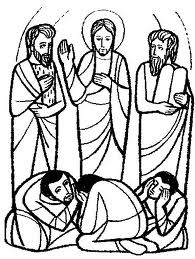
\includegraphics[scale=0.85]{gambar/TRANSFIGURASI.jpeg}
\end{center}
\chap{Banyak yang Terpanggil, Tetapi Sedikit yang Terpilih}

“Dari 44 orang seangkatan yang masuk ke Seminari, akhirnya cuma 6 orang yang ditahbiskan menjadi Imam”.
Sedih dan prihatin mendengar khotbah seorang romo berkaitan dengan jumlah panggilan menjadi imam dewasa ini.
Jujur saja, agak ngeri bila membayangkan suatu saat nanti gereja kita benar2 kehabisan gembala / imam. Bayangkan saja, penambahan jumlah imam yang se ordo dengan imam tersebut, mungkin baru akan terrealisir sekitar 3 atau 4 tahun mendatang. Karena memang dalam kurun waktu 2 sampai dengan 3 tahun mendatang dipastikan tidak akan ada tahbisan imam baru dari ordo tersebut.
Berbagai upaya untuk mengantisipasi hal itu, memang sudah dari dulu di lakukan oleh gereja, baik melalui promosi2 ke beberapa sekolah maupun gereja, juga melalui misa2 dengan tema ‘panggilan’. Namun upaya tersebut ternyata masih belum cukup mampu menjawab tantangan yang dihadapi gereja saat ini, khususnya dalam mendapatkan ‘panggilan-panggilan’ baru.

Kondisi semacam itu sepertinya sudah bisa ditebak bakal terjadi bila melihat realitas yang ada diseputar gereja. Gereja bagaikan berjalan “sendirian” dalam menjala umat yang bersedia mengabdi sebagai imam. Umat terkesan tidak begitu perduli dengan semakin minimnya jumlah “panggilan-panggilan baru”.
Dalam berbagai doa bersama, memang tidak jarang beberapa umat menyuarakan doanya dgn nyaring dan lantang memohon agar jumlah ‘panggilan’ menjadi semakin bertambah. Sekalipun jauh didalam hati kecilnya doa itu sering kali diakhiri dengan kata2 dalam hati, ……”ASAL JANGAN ANAKKU, YA TUHAN”

Masalah krisis imam, bukan saja masalah gereja, tapi adalah masalah kita semua sebagai umat Katolik. Karena pada akhirnya kita jualah yang akan merasakan akibatnya.
Bertitik tolak dari hal diatas, adalah sudah selayaknya kita mulai meningkatkan kepedulian tentang krisis Imam yang sedang melanda gereja kita. Kita mesti lebih meningkatkan dukungan terhadap upaya-upaya gereja dalam menebar benih2 panggilan diantara umat. Kita harus selalu menanamkan SEMANGAT PELAYANAN dengan contoh2 yang nyata, baik dikalangan umat maupun didalam keluarga kita sendiri. Sebab bagaimana mungkin kita mengharapkan mereka bisa berkembang menjadi pribadi2 yang secara total mau menyerahkan seluruh hidupnya menjadi pelayan demi kerajaan Allah, kalau didalam diri mereka tidak pernah ditanamkan SEMANGAT UNTUK MELAYANI. Jangan matikan benih panggilan yang muncul dalam keluarga kita. Justru mesti dipupuk dan dibina agar benih panggilan tersebut tumbuh dengan subur.
Benih ‘panggilan’ seringkali datang dalam keadaan yang samar2. Dan justru di seminarilah para seminaris, hari demi hari hari, bulan demi bulan, tahun demi tahun, mencoba menghayati, memahami, memupuk, memperjelas serta memantapkan panggilannya.
Sebagai umat Katolik, kita mesti meng imani bahwa benih panggilan adalah sebuah karunia Allah yang harus disyukuri. Betapa bahagia dan bangga menjadi sebuah keluarga yang dipilih oleh Allah untuk menerima rahmat adikodrati, yang belum tentu diterimakan kepada keluarga lain, sekalipun mereka memintanya.

Sebagai ‘gereja’ yang sudah dewasa, sudah saatnya kita juga bersikap dewasa dalam iman. Kita harus dukung para imam kita dengan doa dan usaha, bahkan kalau perlu dgn airmata dalam upayanya mempertahankan dan semakin memantabkan ‘panggilan’nya. Jangan biarkan mereka bekerja sendirian sehingga mereka tidak merasa ditinggalkan oleh umatnya. Hentikan rumor2 yang tidak ada dasarnya, berita2 miring yang belum tentu kebenarannya ataupun kritik2 yang tidak membangun/asal2an terhadap para imam kita. Karena hal2 spt itu sama sekali tidak ada manfaatnya bagi kehidupan dan perkembangan gereja.
Seorang imam, bukanlah malaikat, tapi tidak lebih dari seorang manusia biasa juga, yang bisa salah, bisa marah, bisa kecewa, bisa sedih, bisa gagal, dll. Dukungan moril, tenaga dan doa dari umat, tidak saja akan membantu mereka mampu bertahan serta mengatasinya bila hal2 diatas menimpanya, melainkan justru dapat lebih meningkatkan kinerjanya dengan penuh suka cita sebagai seorang gembala yang baik. Sehingga sekalipun mereka hidup dalam KESENDIRIANnya, mereka tetap mampu memberikan “kasih” dan “senyuman” kepada setiap orang.
Mari kita senantiasa berdoa bagi pahlawan2 iman ini agar tetap setia pada panggilannya sampai karya Allah tergenapi di dunia ini.
Sekian dan Tuhan memberkati

\sumber{A. Eddy Irwanto}
\chap{Ordo dalam Gereja Katolik}

Tarekat atau ordo adalah satu kongregrasi dalam Gereja Katolik Roma dimana para anggotanya dari rohaniwan/i, yg terdiri dari biarawan/i di mana mereka mengikat diri dalam kaul (baik sementara maupaun kekal). Selibat dan ketaatan adalah yg paling utama, ketaatan baik terhadap atasan mereka (General Overste), maupun kepada Uskup dan Paus sebagai otoritas GK. Anggota ordo hidup dlm komunitas sosial sesuai dengan tata cara konstitusi dari masing2 kongregasi, atas persetujuan Magisterium Gereja Katolik.
Selain hal tersebut di atas, ada juga institusi sekuler (kaum awam) yang memiliki kongregasi terpisah. (kita pasti pernah mendengar Karmelit Awam...itu salah satu contohnya)

\section*{Ordo}
Komunitas (-komunitas) dengan kaul agung dalam arti luas dengan biara-biara independen (misalnya Benediktin, Trapis); atau dengan biara-biara yang tunduk kepada satu pembesar umum (misalnya Serikat Jesus, Ursulin uni Roma).

\section*{Konggregasi}
Komunitas-komunitas dengan kaul sederhana, tetap atau sementara di bawah satu pembesar umum (misal Serikat Sabda Allah - SVD, Suster Carolus Borromeus - CB)

\section*{Ordo/Konggregasi Klerikal}
Sebagian atau anggota-anggota ditahbiskan imam.
Awam: semua anggota tidak ditahbiskan imam.

\section*{Aneka Ordo Pria}
\textit{Ordo Rahib} yang anggota-anggotanya terikat pada satu biara dan menjalankan hidup kontemplatif (a.l. Ordo Benediktin dengan Ordo Sistersien dan Trapis, Ordo Kartusian).

\textit{Ordo Kanonik Reguler} menghimpun imam-imam yang membentuk dewan katedral atau dewan gereja yang hidup menurut aturan tentang dan terikat doa ofisi bersama (antara lain Ordo Kanonik S. Agustinus, Ordo Salib Suci)

\textit{Ordo Kesatria atau Hospital} melindungi milik apapun, maka dahulu mencari rejeki dengan mengemis (antara lain Ordo Fransiskan dan Klaris serta Kapusin, ordo Dominikan, Karmelit)

\textit{Ordo Kleris} dengan regula, yang melepaskan doa ofisi bersama, hidup dalam biara dan pakaian biarawan, supaya lebih bebas berkarya pada saja dan di mana pun diperlukan, baik secara sendiri maupun bersama (antara lain Serikat Jesus).

\section*{Ordo Wanita}
\noindent{Ordo Rubiah -- Benediktin (termasuk Trapis)\\
Ordo Kedua Pengemis -- Klaris, Kapusines, Karmelites\\
Ordo Biarawati aktif -- Ursulin}

\section*{Para Imam}

Dalam Gereja Katolik imam merupakan jabatan tetap,
melalui proses pendidikan  dan pemberkatan  (tahbisan,
penerimaan Sakramen Tahbisan). Yang bisa menjadi imam
hanyalah laki-laki.  Imam juga tidak
diperbolehkan untuk menikah (hidup selibat), seumur hidup.
Begitu seorang imam menikah, maka jabatan imamatnya harus
dilepaskan. 

Yang bisa memimpin ibadat misa dan memberikan sakramen
hanyalah imam yang sah. Dalam keadaan imam tidak
ada, maka ibadat misa ditiadakan dan diganti dengan ibadat
sabda yang bisa dipimpin oleh bukan imam. 

Di Jawa para imam biasa disapa dengan panggilan
``\textit{romo}'', yang artinya bapak. Ini merupakan terjemahan
harafiah dari sapaan imam di Eropa yang dipanggil \textit{pater}, atau
\textit{father}, yang juga bermakna bapak. Para imam yang mengelola
sebuah paroki, lazim disebut pastor, yang berasal dan bahasa
Latin dengan arti gembaIa. Imam kepala di sebuah paroki,
disebut sebagai pastor kepala. Namun sekarang semua imam,
meskipun tidak mengelola sebuah paroki, juga disapa dengan
panggilan pastor. Bahkan di beberapa negara, pendeta Kristen/
Protestan pun disapa dengan panggilan pastor. 


\section*{10 Tarekat Pria Terbesar di Dunia}

\begin{tabular}{llrr}
\hline
&\textbf{Tarekat}&\textbf{Anggota}&\textbf{Imam}\\
\hline
1.	&SJ (Jesuit) 		&21.490	&15.105\\
2.	&OFM (Fransiskan)	&17.335	&11.417\\
3. 	&SDB (Salesian)		&17.192	&11.224\\
4.	&OFMCap (Kapusin)	&11.303	&7.303\\
5.	&OSB (Benediktin)	&7.926	&4.565\\
6.	&OP (Dominikan)		&6.375	&4.768\\
7.	&SVD (Sabda Ilahi)	&5.962	&3.769\\
8.	&CSsR (Redemptoris)	&5.773 	&4.262\\
9.	&OMI (Oblat)		&4.831	&3.508\\
10.	&OFMConv. (Konventual)	&4.499	&2.783\\
\hline
\end{tabular}

\section*{10 Tarekat Pria Terbesar di Indonesia}

\begin{tabular}{llrr}
\hline
&\textbf{Tarekat}&\textbf{Anggota}&\textbf{Imam}\\
\hline
1.	&SVD 	&947	&440\\
2.	&SJ 	&338	&238\\
3.	&OFMCap	&335	&178\\
4.	&MSC	&322	&183\\
5.	&OCarm 	&201	&93\\
6.	&OFM 	&194	&75\\
7.	&MSF	&181	&100\\
8.	&SCJ	&177	&103\\
9.	&OSC	&135	&85\\
10.	&CM		&123 	&76\\
\#	&Praja	&2.502	&1.177\\ \hline
\end{tabular}

Di seluruh Indonesia, ada 26 ordo (konggregasi, tarekat) imam Katolik, dan imam projo (diosesan). Masing-masing ordo seakan-akan punya wilayah tersendiri. Misalnya SVD lebih banyak berkarya di NTT, OFMCap di Kalbar dan Sumut, Jesuit di Jateng (minus Purwokerto), DIY, dan DKI Jakarta. Imam Projo, yang langsung berada di bawah uskup dan tidak menjadi anggota ordo, menyebar di keuskupan masing-masing, terutama keuskupan di Jawa. Imam yang anggota tarekat maupun iman projo, tidak hanya bertugas di paroki (gereja), atau di biara masing-masing, melainkan juga berkarya di luar tarekat/keuskupan. Di antara mereka ada yang mengelola kegiatan gereja (sekolah, perguruan tinggi, penerbitan), ada pula yang berkarya di instansi pemerintah. Misalnya pastor tentara, yang bertugas di kesatuan/angkatan.

\section*{Imam Katolik di Indonesia}

\begin{enumerate}
\item Imam praja/diosesan (Pr)
\item Ordo Karmel (O Carm; Karmelit)
\item Ordo Saudara-saudara Dina (OFM; Fransiskan)
\item Ordo Salib Suci (OSC)
\item Ordo S. Agustinus (OSA)
\item Ordo Saudara-saudara Dina Konventual (OFM Conv.)
\item Ordo Saudara-saudara Dina Kapusin (OFM Cap.)
\item Serikat Jesus (SJ, Jesuit)
\item Ordo Karmel Tak Berkasut (OCD)
\item Ordo Trapis (OCSO)
\item Kongregasi Misi (CM, Lazaris)
\item Serikat Imam Misi Luar Negeri (Paris-MEP)
\item Serikat Maria Monfortan (SMM)
\item Kongregasi Sengsara Yesus (CP; Pasionis)
\item Kongregasi Redemptoris (CSsR)
\item Kongregasi Pater-pater Hati Kudus Yesus dan Maria(SSCC; Picpus)
\item Kongregasi S.  Perawan  Maria Yang Terkandung TakBernoda (OMI; Oblat)                      
\item Kongregasi Misionaris Hati Kudus (MSC)
\item Serikat Salesian Don Bosco (SDB)
\item Kongregasi Hati Maria Tak Bernoda (CICm; Scheutis)
\item Misionaris Mill Hill (MHM)
\item Serikat Sabda Allah (SVD)
\item Kongregasi Imam-imam Hati Kudus Yesus (SCJ)
\item Kongregasi Misionaris Keluarga Kudus (MSF)
\item Serikat S. Fransiskus Xaverius (SX; Xaverian)
\item Misionaris Maknoll (MM)
\item Kongregasi Murid-murid Tuhan (CDD)
\end{enumerate}

%\chap{Senyum Sejenak}

\setlength{\parindent}{0cm}
\section*{Bercanda}
\begin{itemize}
\item[Cewek:] Mulai hari ini kita putus!
\item[Cowok:] Kok begitu... (kaget), padahal besok aku mau belikan kamu HP yang mahal.
\item[Cewek:] Hm... (mikir-mikir), aku hanya bercanda kok, Sayang.
\item[Cowok:] Oh, sama. Aku juga bercanda.
\end{itemize}

\kutipan{"Tak bergunalah dan jahatlah orang yang hidup dengan mulut serong."\\
(Amsal 6:12)
}

\section*{Menanyai seorang angkatan laut muda}

Seorang kapten kapal laut memberi beberapa pertanyaan kepada seorang 
angkatan laut muda. \\
"Apa yang kamu lakukan jika tiba-tiba ada badai?"\\
"Aku akan melemparkan jangkar, Pak."\\
"Apa yang kamu lakukan jika ada badai datang lagi?"

"Aku akan melempar jangkar lain, Pak."

"Nah, terus bagaimana jika ada badai ketiga yang menyerang?"

"Aku akan melemparkan jangkar lain, Kapten."

"Tunggu dulu, Nak. Dari mana kamu dapat jangkar sebanyak itu?"

"Dari tempat yang sama di mana Anda mendapatkan semua badai itu, Pak."

\kutipan{"Karena sebagaimana mimpi disebabkan oleh banyak kesibukan, demikian 
pula percakapan bodoh disebabkan oleh banyak perkataan." \\
(Pengkhotbah 5:3)}
\setlength{\parindent}{1cm}
\normalsize
\chap{Warta Lingkungan}

\subsection*{APP}
Bulan Maret 2012 sudah masuk dalam masa Prapaskah. Sesuai dengan tradisi, setiap masa Prapaskah diadakan Aksi Puasa Pembangunan yang kegiatannya antara lain adalah ibadat APP di lingkungan. Untuk tahun ini Keuskupan Agung Semarang (KAS) menetapkan tema APP: \textit{Umat Katolik Sejati Harus Peduli dan Berbagi}. Dalam pelaksanaan di lingkungan St. Petrus, ibadat APP banyak diisi dengan \textit{sharing} yang mengacu pada buku panduan dari KAS.
Topik APP berawal dari baptis. Kapan kita dibaptis, kesan-kesan saat dibaptis, dan relevansinya dengan hidup menggereja dan bermasyarakat.

\subsection*{Misa pemberkatan rumah dan mitoni}
Bulan ini umat St. Petrus bertambah lagi dengan satu keluarga yang secara resmi bergabung sebagai warga lingkungan. Keluarga Bapak R. Mulyadi yang bertempat tinggal di Nanggulan, mengadakan misa syukur pemberkatan rumah dan sekaligus mitoni pada tanggal 22 Maret. Cicilia Nony Prayoga yang merupakan putri dari Bapak/Ibu Mulyadi menantikan kelahiran putranya bersama dengan suami tercinta
Bernadus Budhiprayoga.

Misa dipimpin oleh Rm. Albertus Purnomo, OFM yang merupakan kenalan baik keluarga R. Mulyadi saat masih di Jakarta. Dalam homilinya Romo menekankan bahwa Musa dapat melakukan tawar-menawar dengan Tuhan karena kedekatan Musa dengan Tuhan. Kenapa Musa dekat dengan Tuhan, karena Musa sering berdoa dan menaati perintah-Nya. Oleh karena itu kalau kita ingin dekat dengan Tuhan, maka rajin-rajinlah berdoa dan senantiasa menaati perintah-Nya.

\subsection*{Pendaftaran Krisma}
Telah diumumkan di gereja bahwa sakramen Krisma untuk paroki Marganingsih Kalasan akan dilangsungkan bulan September 2012. Calon penerima sakramen Krisma dapat mendaftarkan diri ke Ibu Munarti, Bapak Neo Suradi, atau kepada ketua lingkungan, dengan menyerahkan fotokopi surat baptis.

% SELECT day(`TglLahir`),
% concat(u1.`Baptis`,' ',u1.`Nama`) 
% FROM `umat` u1 WHERE month(TglLahir)=6 order by 1

%=========
% SELECT day(`TglNikah`),
% concat(u1.`Baptis`,' ',u1.`Nama`,' + ',u2.`Baptis`,' ',u2.`Nama`) 
% FROM `umat` u1 join kk on (u1.nokk=kk.id and u1.hubkel='KK')
%               join umat u2 on (u2.nokk=kk.id  and (u2.hubkel='istri' or u2.hubkel='isteri'))
% WHERE month(TglNikah)=1 order by 1

\section*{Yang berulang tahun kelahiran bulan ini}

\noindent{Semoga hari bahagia ini menguatkan imannya akan Dikau.}

\begin{longtable}{|c|l|} 
\hline
Tgl & Nama \\ \hline
\endhead1& Maria Rosary Sekar Seruni\\
5& Anna Maria Tri Henaningsih\\
6& Fransiscus Xaverius Sularto\\
7& Christina Sutarni\\
8& Marcellina Oktavia S. Padmini\\
11& Priscilla Oktiva Rossari\\
15& Yoseph Laba Atawolo\\
16& Ignatius Stanley Andi Pradana\\
18& Christina Sri Ning Hastuti\\
24& Margareta Maria Sri Pramuwati\\
25& Kristina Tri Tutwuri\\
\hline
\end{longtable}



\section*{Yang berulang tahun perkawinan  bulan ini}

Selamat ulang tahun perkawinan. Semoga keluarga-keluarga ini tumbuh menjadi keluarga Katolik yang sejati yang dibangun atas dasar iman dan kasih: kasih akan Dikau dan kasih antar semua anggota keluarga.

\begin{longtable}{|c|l|} 
\hline
Tgl & Keluarga \\ \hline
\endhead5& Nikolas Putut Andoko + Chatarina Krisyanti\\
6& Ignatius Luddy Indra Purnama + Anna Sri Wuryaningtyas\\
\hline
\end{longtable} 

\newpage
\chap{Kompendium Katekese Gereja Katolik}
\setcounter{kgkcounter}{49}
\small
\kgk{Apa artinya mengatakan bahwa Allah itu mahakuasa?}
      Allah mewahyukan diri-Nya sebagai ”Dia yang kuat, Dia yang kuasa” (Mzm     268-278
24:8), sebagai Dia ”yang bagi-Nya tidak ada yang mustahil” (Luk 1:37). Kemahakuasaan-Nya itu universal, gaib, dan yang menunjukkan Diri-Nya di dalam
penciptaan dunia dari ketiadaan dan penciptaan manusia dari cinta, tetapi ter-
utama menunjukkan Diri-Nya dalam Penjelmaan dan Kebangkitan Putra-Nya,
dalam anugerah pengangkatan anak dan dalam pengampunan dosa-dosa. Karena
hal inilah, Gereja mengalamatkan doa-doanya kepada ”Allah yang mahakuasa dan
kekal” (”Omnipotens sempiterne Deus ...”).

\kgk{Apa pentingnya mengatakan, ”Pada awal mula, Allah menciptakan
    langit dan bumi” (Kej 1:1)?}
     Maknanya, penciptaan itu dasar dari semua rencana penyelamatan Allah.       
Tindakan penciptaan itu menunjukkan kekuasaan dan cinta bijaksana Allah,        
merupakan langkah pertama menuju kepada perjanjian antara Allah dengan
umat-Nya. Penciptaan merupakan permulaan sejarah keselamatan yang memuncak dalam diri Kristus, dan jawaban pertama terhadap pertanyaan dasar kita mengenai asal dan tujuan akhir.

          \kgk{Siapa yang menciptakan dunia?}
Bapa, Putra, dan Roh Kudus adalah prinsip penciptaan yang satu dan tak
terpisahkan walaupun karya penciptaan dunia secara khusus dikenakan kepada
          Allah Bapa.

\kgk{Mengapa dunia diciptakan?}
Dunia diciptakan bagi kemuliaan Allah yang ingin menunjukkan dan
mengomunikasikan kebaikan, kebenaran, dan keindahan-Nya. Tujuan akhir penciptaan, Allah menjadi ”semua di dalam semua” dalam Diri Kristus (1Kor 15:28)
          untuk kemuliaan-Nya dan kebahagiaan kita.


\flushright{(\dots \emph{bersambung} \dots)}
\normalsize
\end{document}